% Generated by source/book_tour.py; do not edit by hand.
\chapter{Usage scenarios}
\label{ch:usage}
These screenshots come from the running application, driven by a script that plays the parts of three people: alice creates the challenge, bob joins her, and carol watches. \texttt{make tour} in the project root reproduces them; \path{book/assets/tour/manifest.json} records each step, viewer, image hash, source hashes and browser version. Bot moves come from a time-limited search, so the stones differ between runs while the steps do not.

\section{Welcome}
A visitor chooses a local display name. Nothing else is needed for the local preview.

\begin{figure}[ht]
\centering
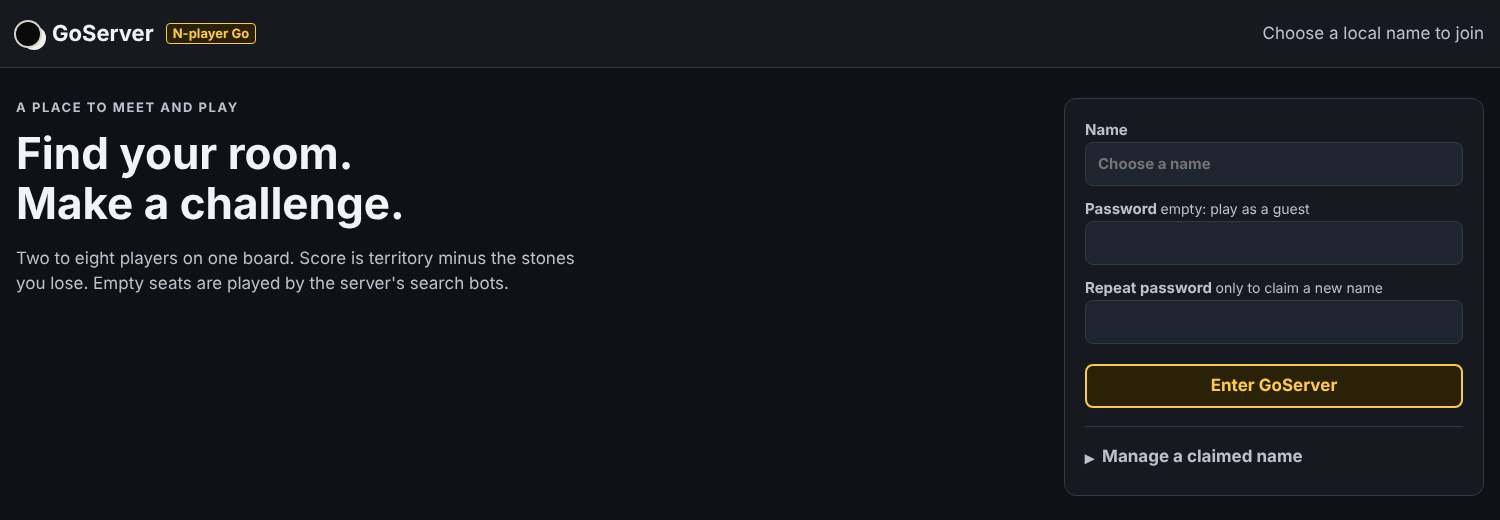
\includegraphics[width=\textwidth]{assets/tour/01-welcome.png}
\caption{Welcome, seen by alice. Steps: open the app.}
\end{figure}
\clearpage

\section{Creating a challenge}
Alice is in the lobby and fills in a challenge: a 9$\times$9 board, three players, and a byo-yomi clock of one minute of main time and then three periods of ten seconds, the same for people and bots. The ko rule stays on Auto, which is off for three players.

\begin{figure}[ht]
\centering
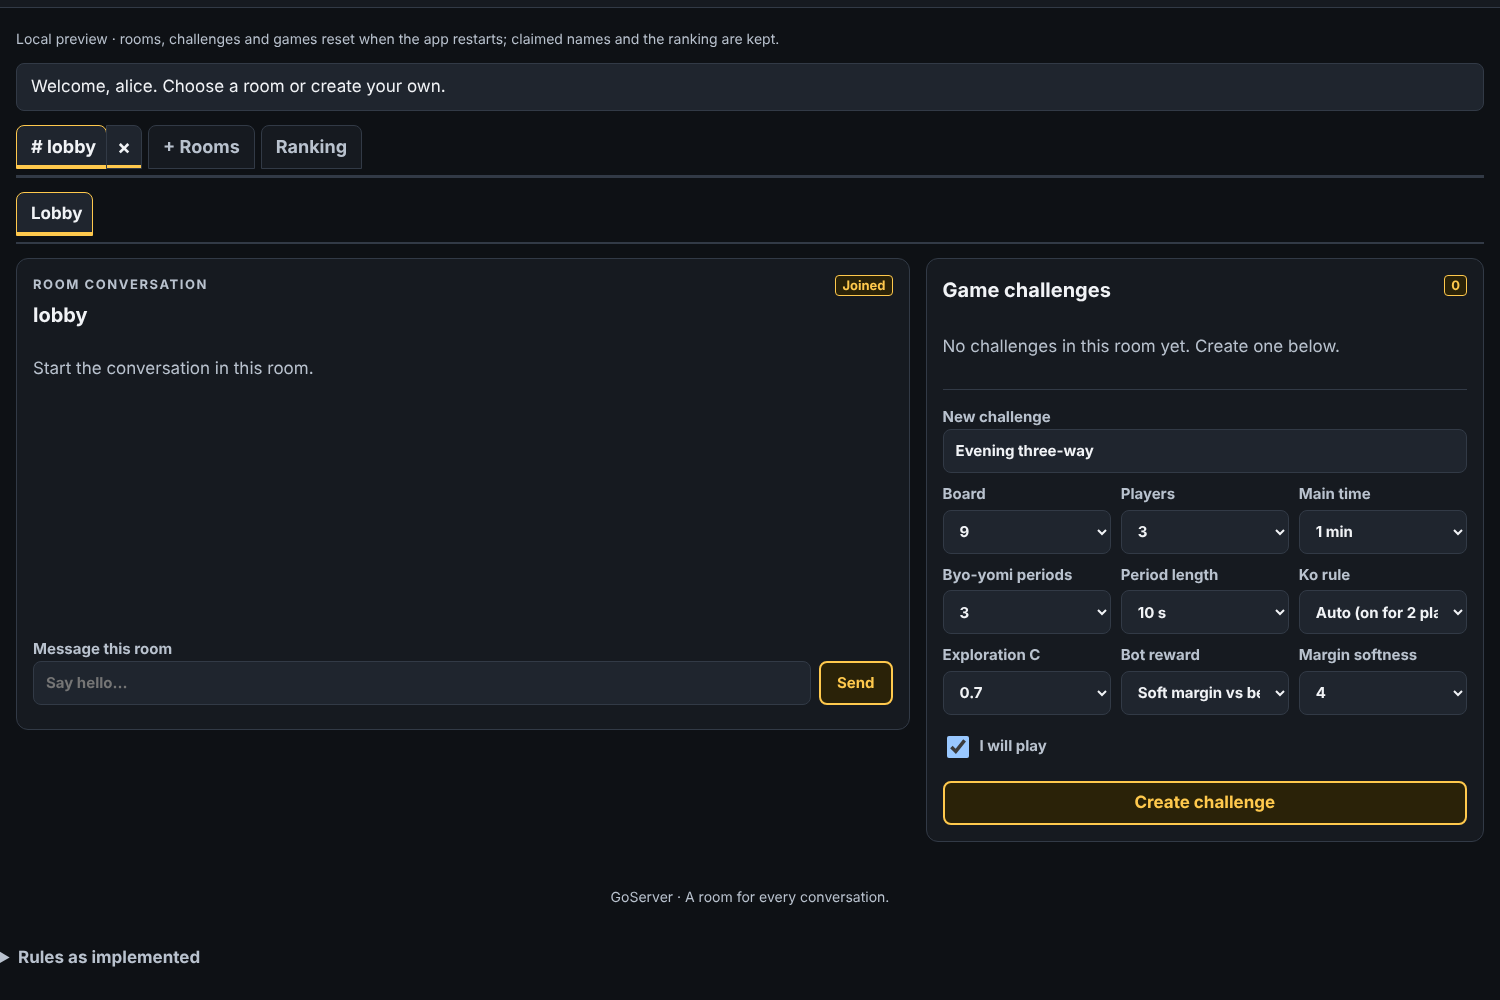
\includegraphics[width=\textwidth]{assets/tour/02-create-challenge.png}
\caption{Creating a challenge, seen by alice. Steps: sign in as alice; fill in the New challenge form.}
\end{figure}
\clearpage

\section{Planning seats}
Before the start the creator decides, seat by seat, whether a person or a bot plays and which team the seat is on. Alice took seat 1, bob sat in seat 2, and alice marked seat 3 as a bot.

\begin{figure}[ht]
\centering
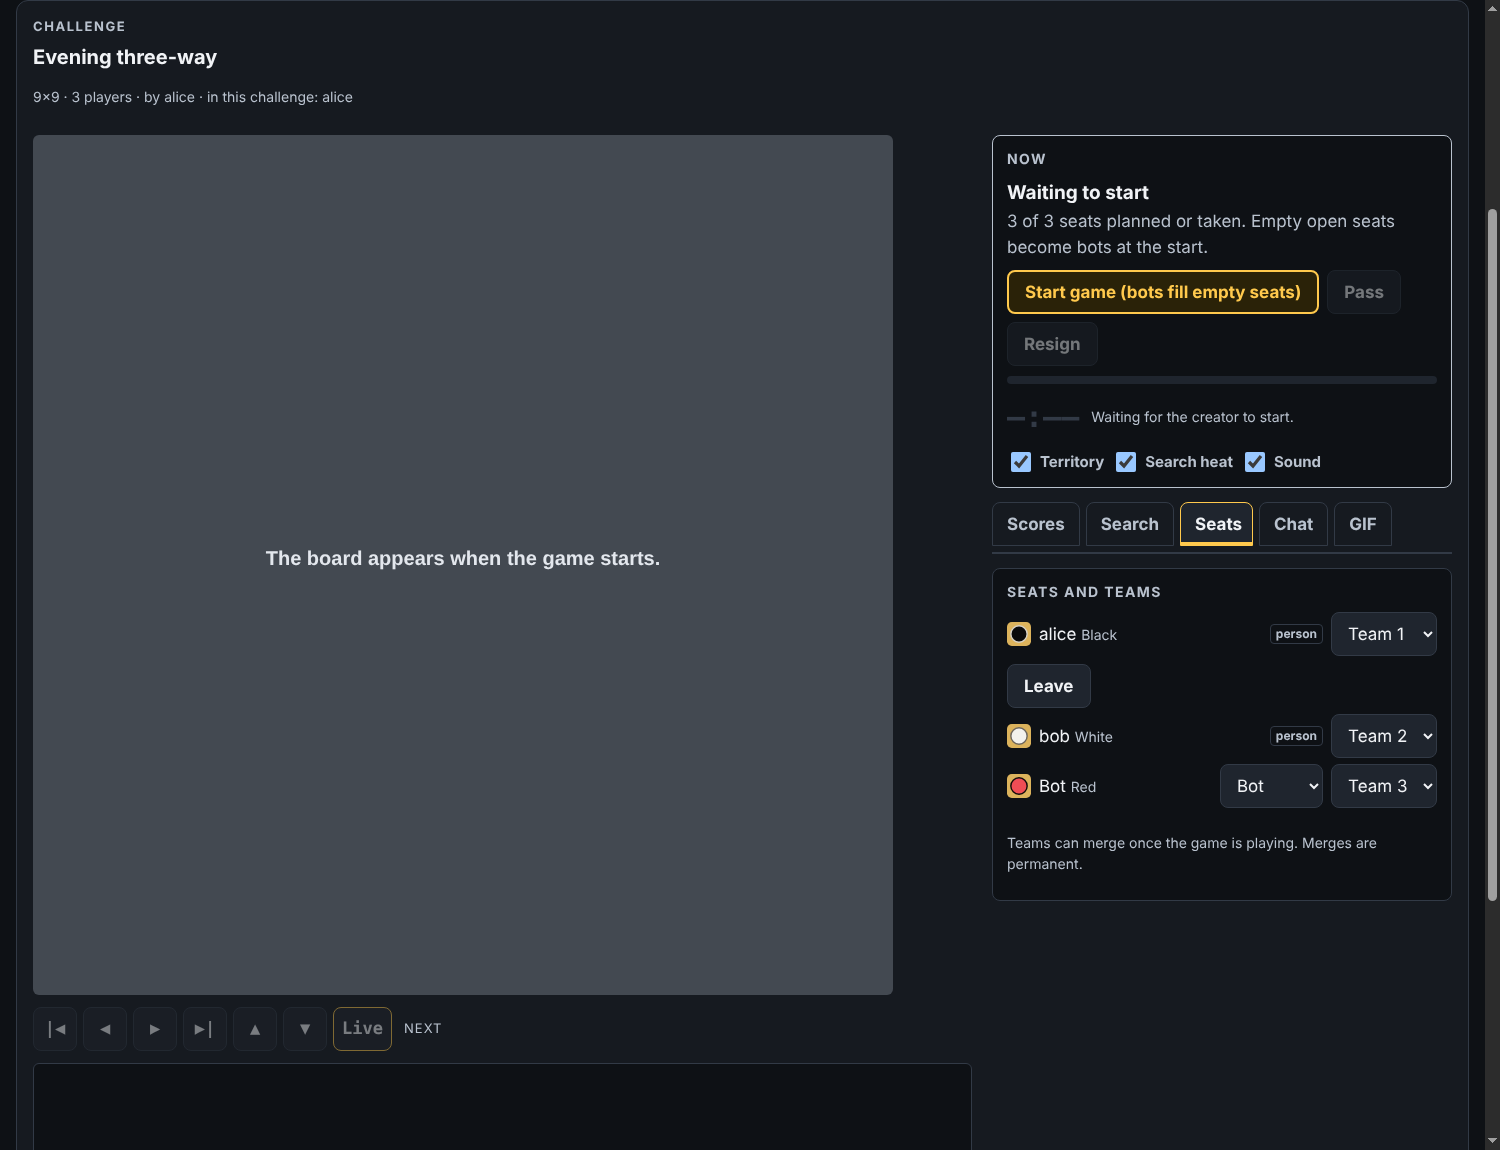
\includegraphics[width=\textwidth]{assets/tour/03-seat-plan.png}
\caption{Planning seats, seen by alice. Steps: alice: create the challenge (seated automatically); alice: set seat 3 to Bot; bob: open the challenge, Sit here.}
\end{figure}
\clearpage

\section{Aiming a stone}
On her turn alice moves the pointer over the board: a translucent stone in her colour shows exactly where a click will play. Over an occupied point, a point the ko rule forbids, or when it is not her turn, there is no preview and the pointer shows that a click would be refused. Above the tabs, the play bar keeps whose turn it is and the clock in view.

\begin{figure}[ht]
\centering
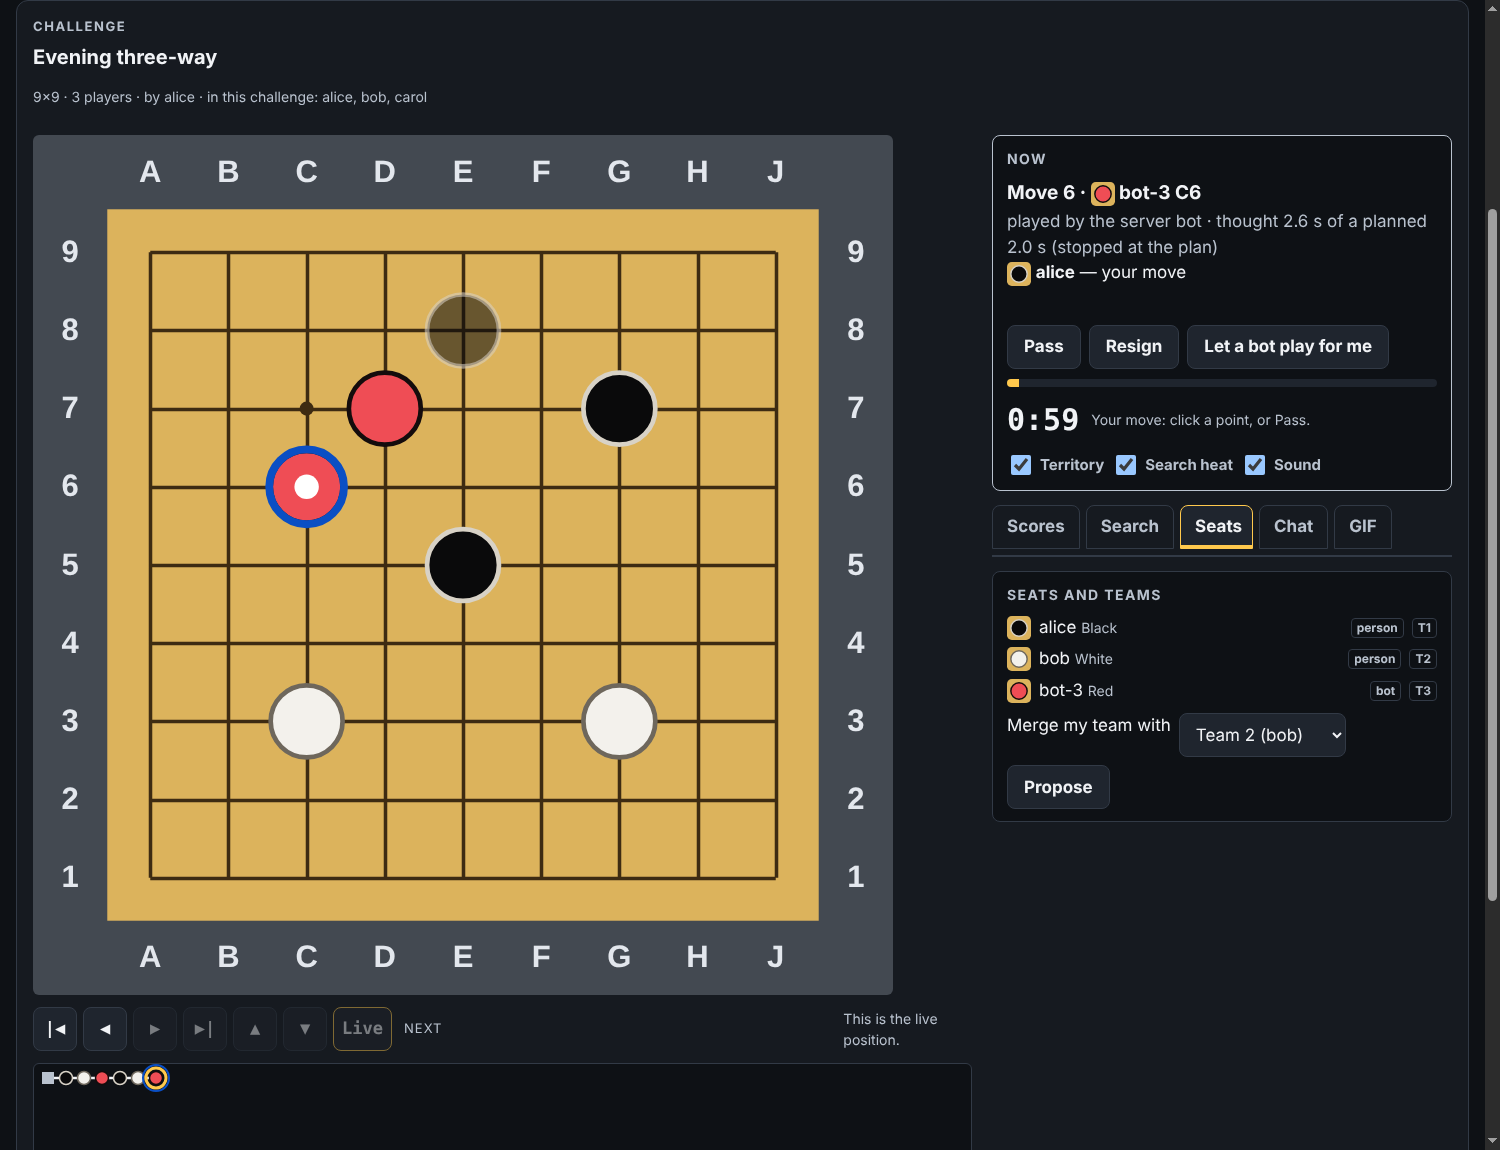
\includegraphics[width=\textwidth]{assets/tour/04a-aim.png}
\caption{Aiming a stone, seen by alice. Steps: alice: move the pointer over an empty point on her turn.}
\end{figure}
\clearpage

\section{Reading the bot's search}
Alice steps back one move, to the position where the bot searched for its last move. The panel lists the moves that search weighed, with visit share and expected reward; the blue discs on the board are the same search as a heat map. Proj. and Outlook give every seat's projected final score and expected reward, and the timeline under them plots the projections move by move.

\begin{figure}[ht]
\centering
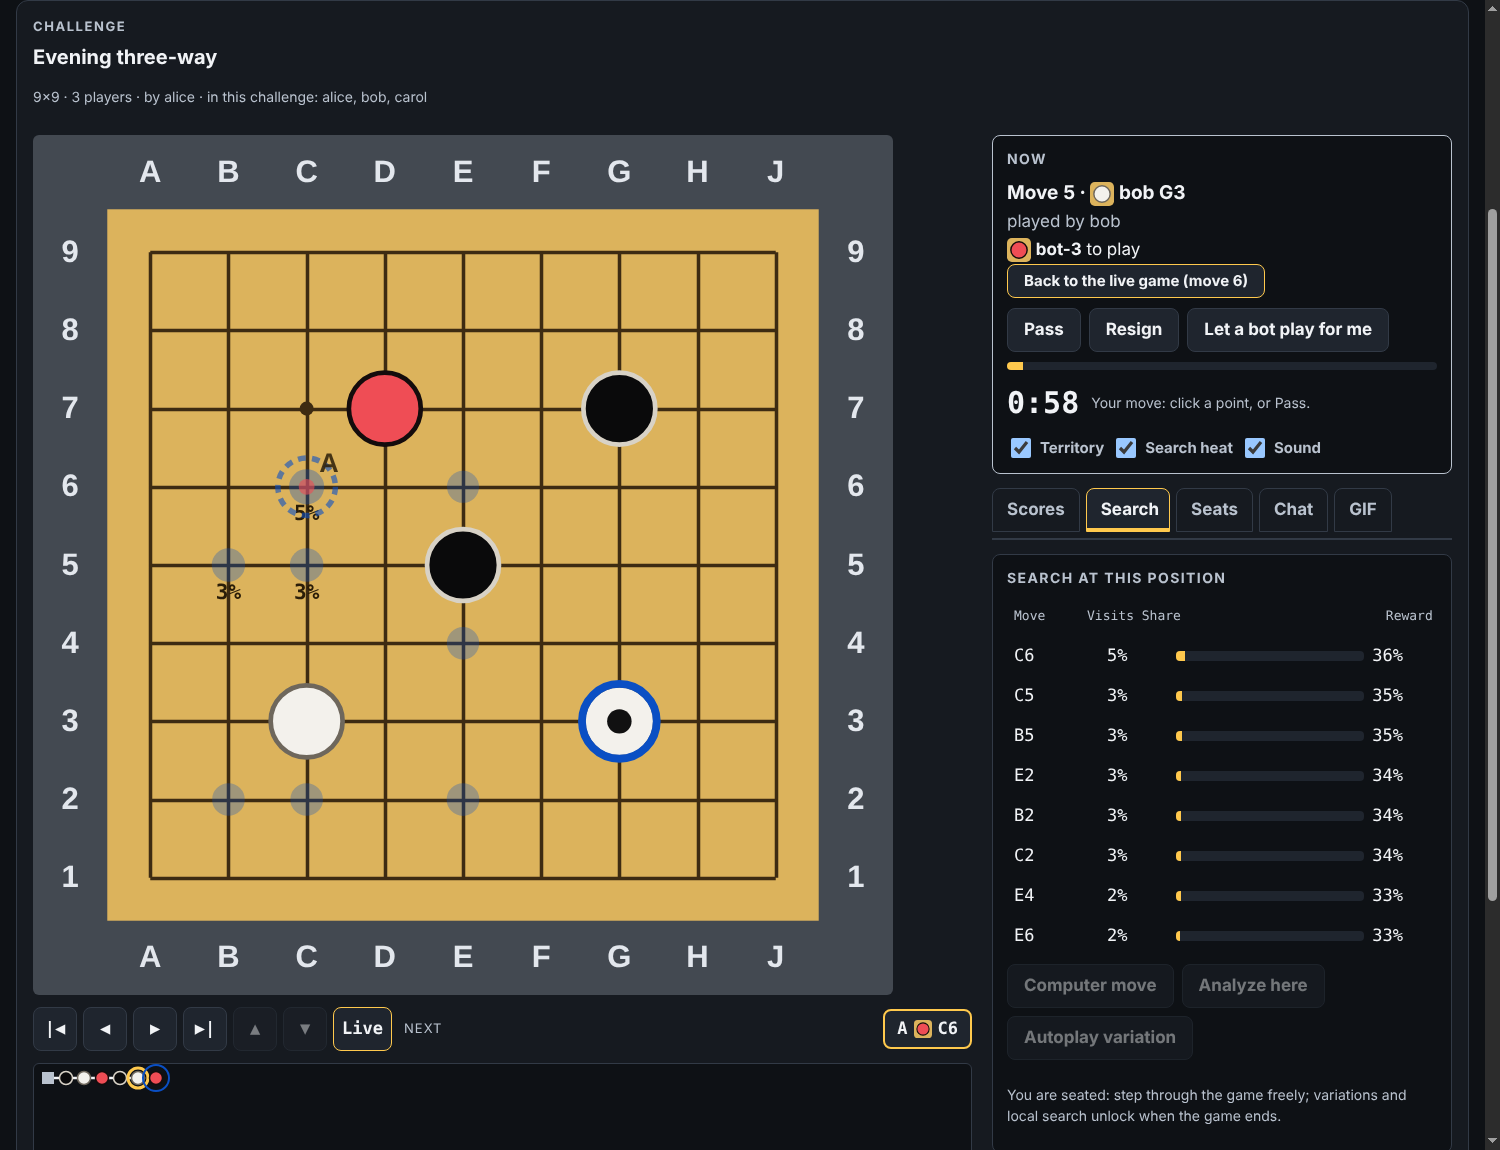
\includegraphics[width=\textwidth]{assets/tour/04-bot-search.png}
\caption{Reading the bot's search, seen by alice. Steps: alice and bob alternate stones by clicking the board; the bot answers each round; alice: Back one move.}
\end{figure}
\clearpage

\section{A watcher explores a variation}
Carol is watching, not playing. She steps back to move 3, tries a different stone (the gold ring marks a variation), and asks for a local search. The analysis runs in her browser only: the dashed branch in the tree never reaches the server, and the live game continues.

\begin{figure}[ht]
\centering
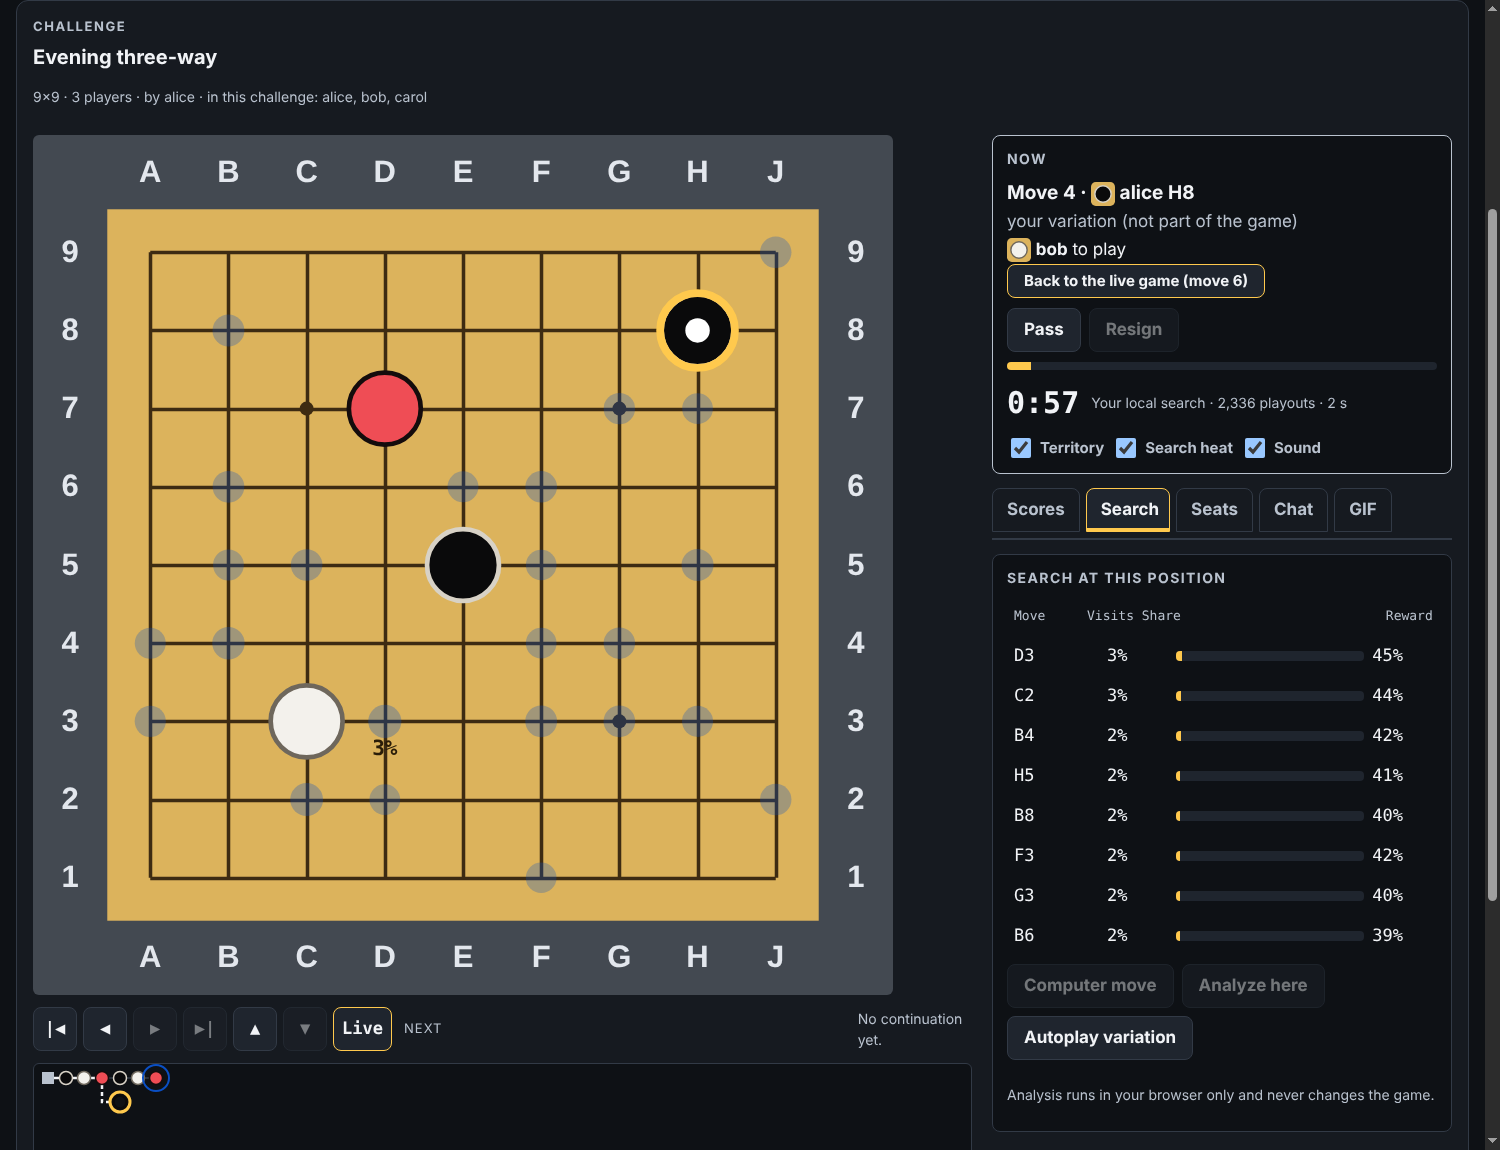
\includegraphics[width=\textwidth]{assets/tour/05-watcher-variation.png}
\caption{A watcher explores a variation, seen by carol. Steps: carol: open the challenge as a watcher; carol: Home, then Forward three times; carol: click an empty point; carol: Analyze here.}
\end{figure}
\clearpage

\section{Proposing a team merge}
During play bob proposes merging his team with alice's. The Seats tab flags a proposal waiting for her answer; there the proposal shows who has accepted and who is still to answer; it takes effect only when every person on both teams accepts, and it is permanent.

\begin{figure}[ht]
\centering
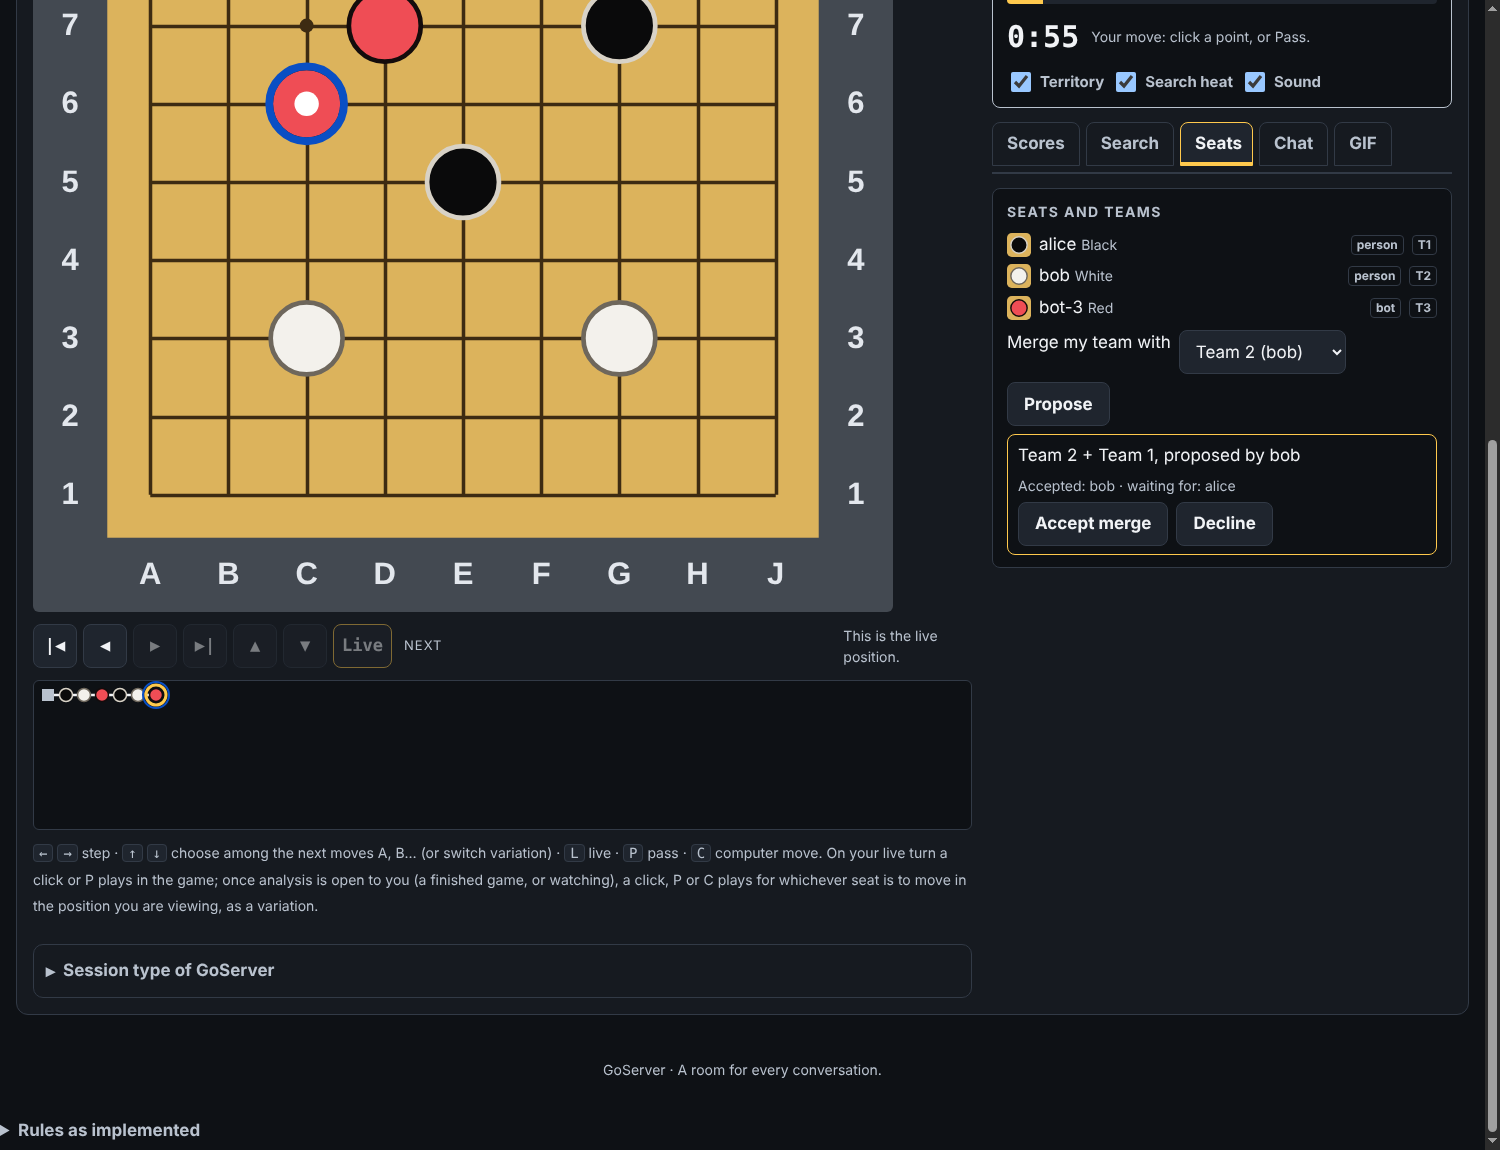
\includegraphics[width=\textwidth]{assets/tour/06-merge-proposal.png}
\caption{Proposing a team merge, seen by alice. Steps: bob: Merge my team with Team 1, Propose.}
\end{figure}
\clearpage

\section{Playing as a team, on autopilot}
After the merge the score table shows alice and bob as team 1 with a combined total. Alice then lets a bot play her seat; the seat, team and name stay hers, and the bot's move publishes its search like any other bot move. She can take the seat back at any time.

\begin{figure}[ht]
\centering
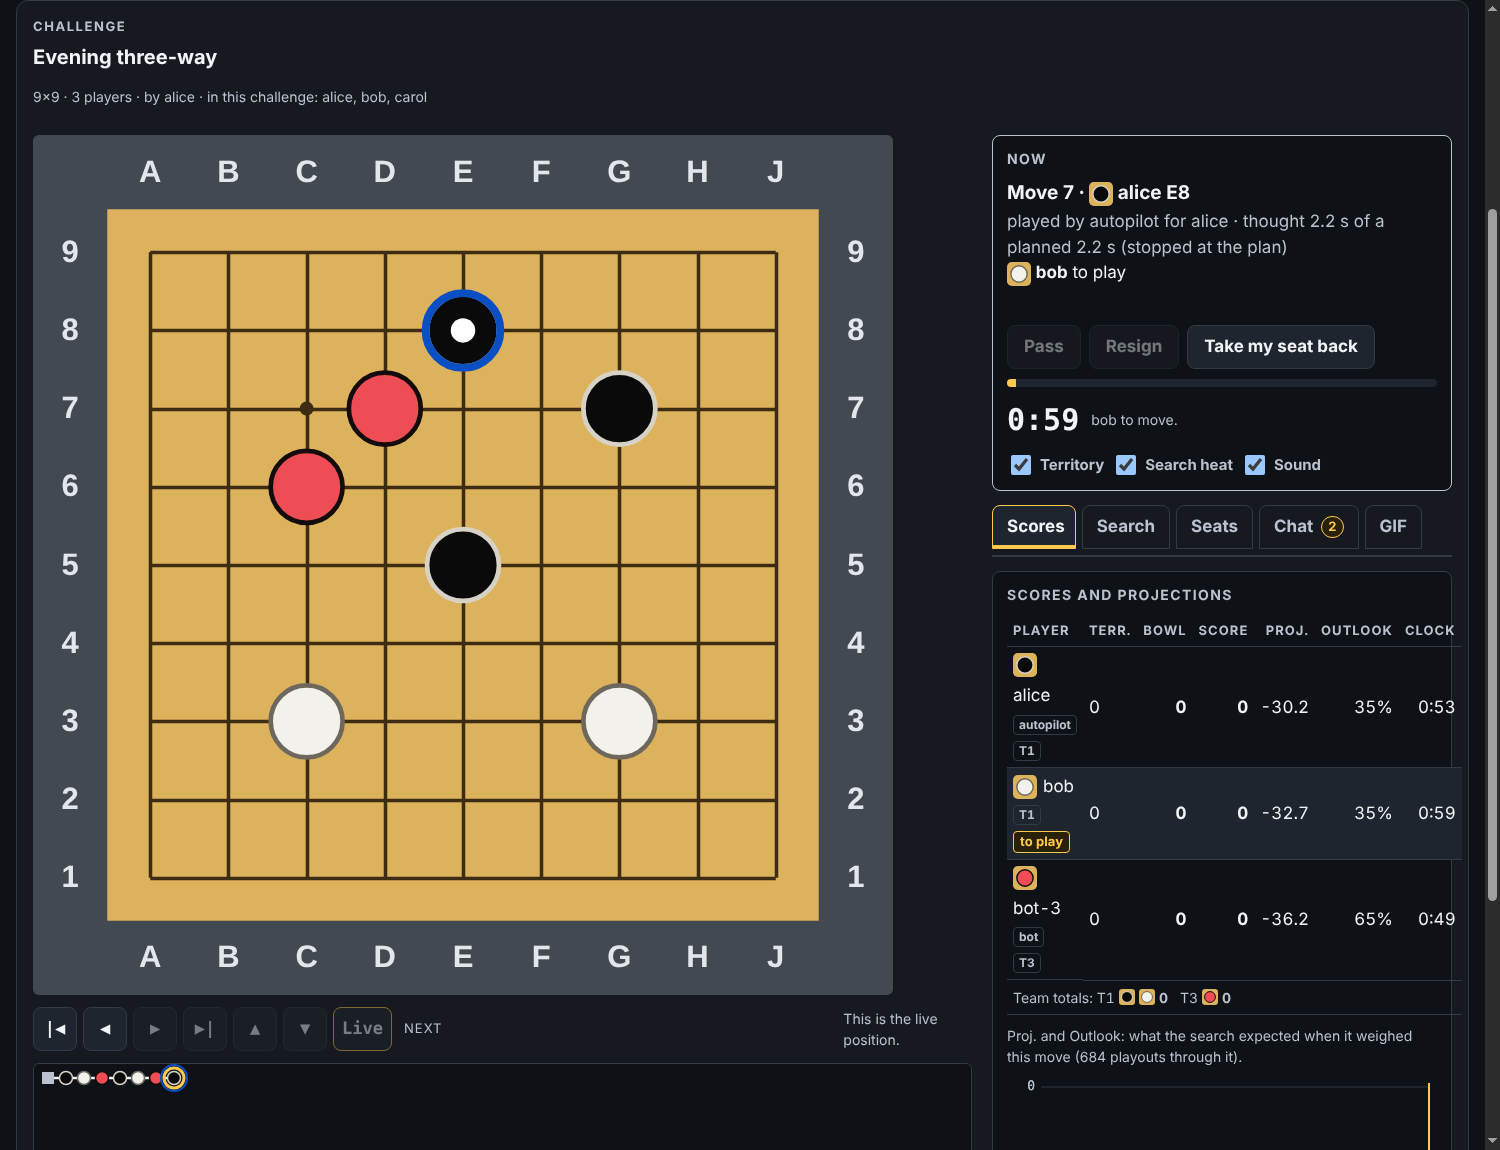
\includegraphics[width=\textwidth]{assets/tour/07-team-and-autopilot.png}
\caption{Playing as a team, on autopilot, seen by alice. Steps: alice: Accept merge; alice: Let a bot play for me.}
\end{figure}
\clearpage

\section{The result}
When every remaining player has passed in a row the game ends. The Chat tab lights up with an unread count; the server announces team scores and the winners in the game conversation. Everyone, players included, can now branch and analyse any position.

\begin{figure}[ht]
\centering
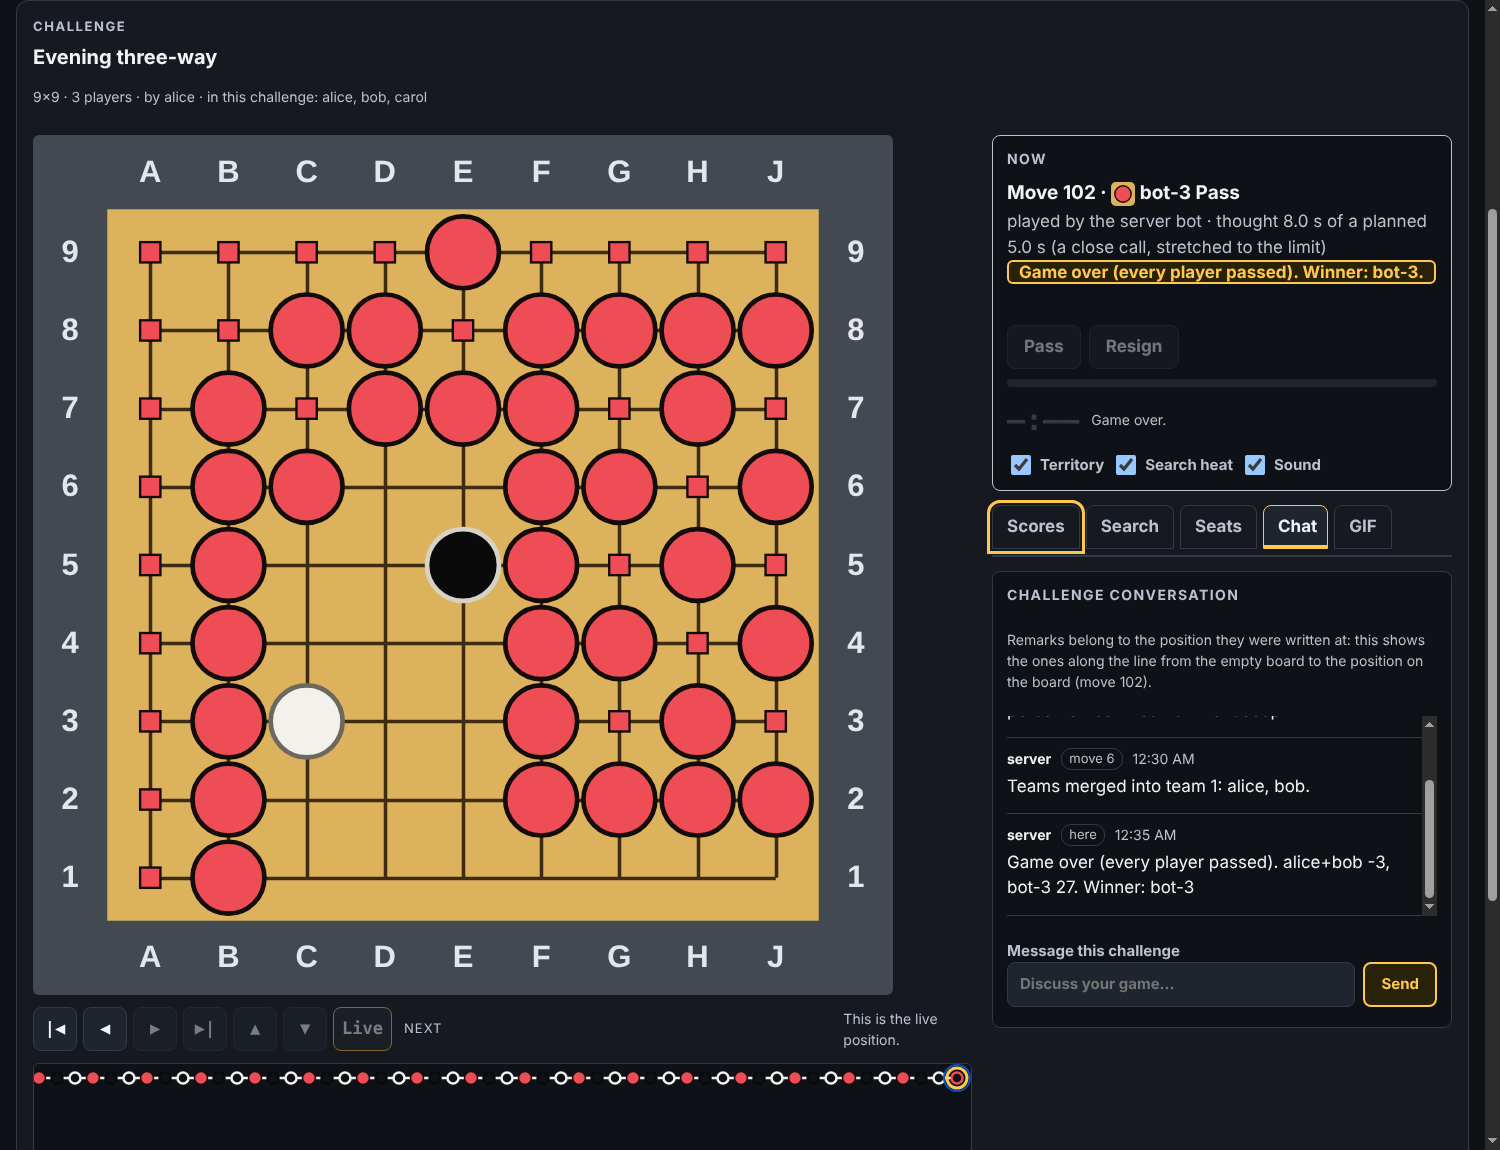
\includegraphics[width=\textwidth]{assets/tour/08-game-over.png}
\caption{The result, seen by alice. Steps: alice passes with the P key, bob with the Pass button, until the bot also passes.}
\end{figure}
\clearpage

\section{Reviewing together}
After the game alice steps back to move 2, passes for the seat to move there and lets the computer pick the next move. Both moves are kept on the server for everyone in the game, and her remark is pinned to the position she was looking at: the Chat tab shows the remarks along the line on the board, so stepping back hides it again and anyone who walks into this variation sees it.

\begin{figure}[ht]
\centering
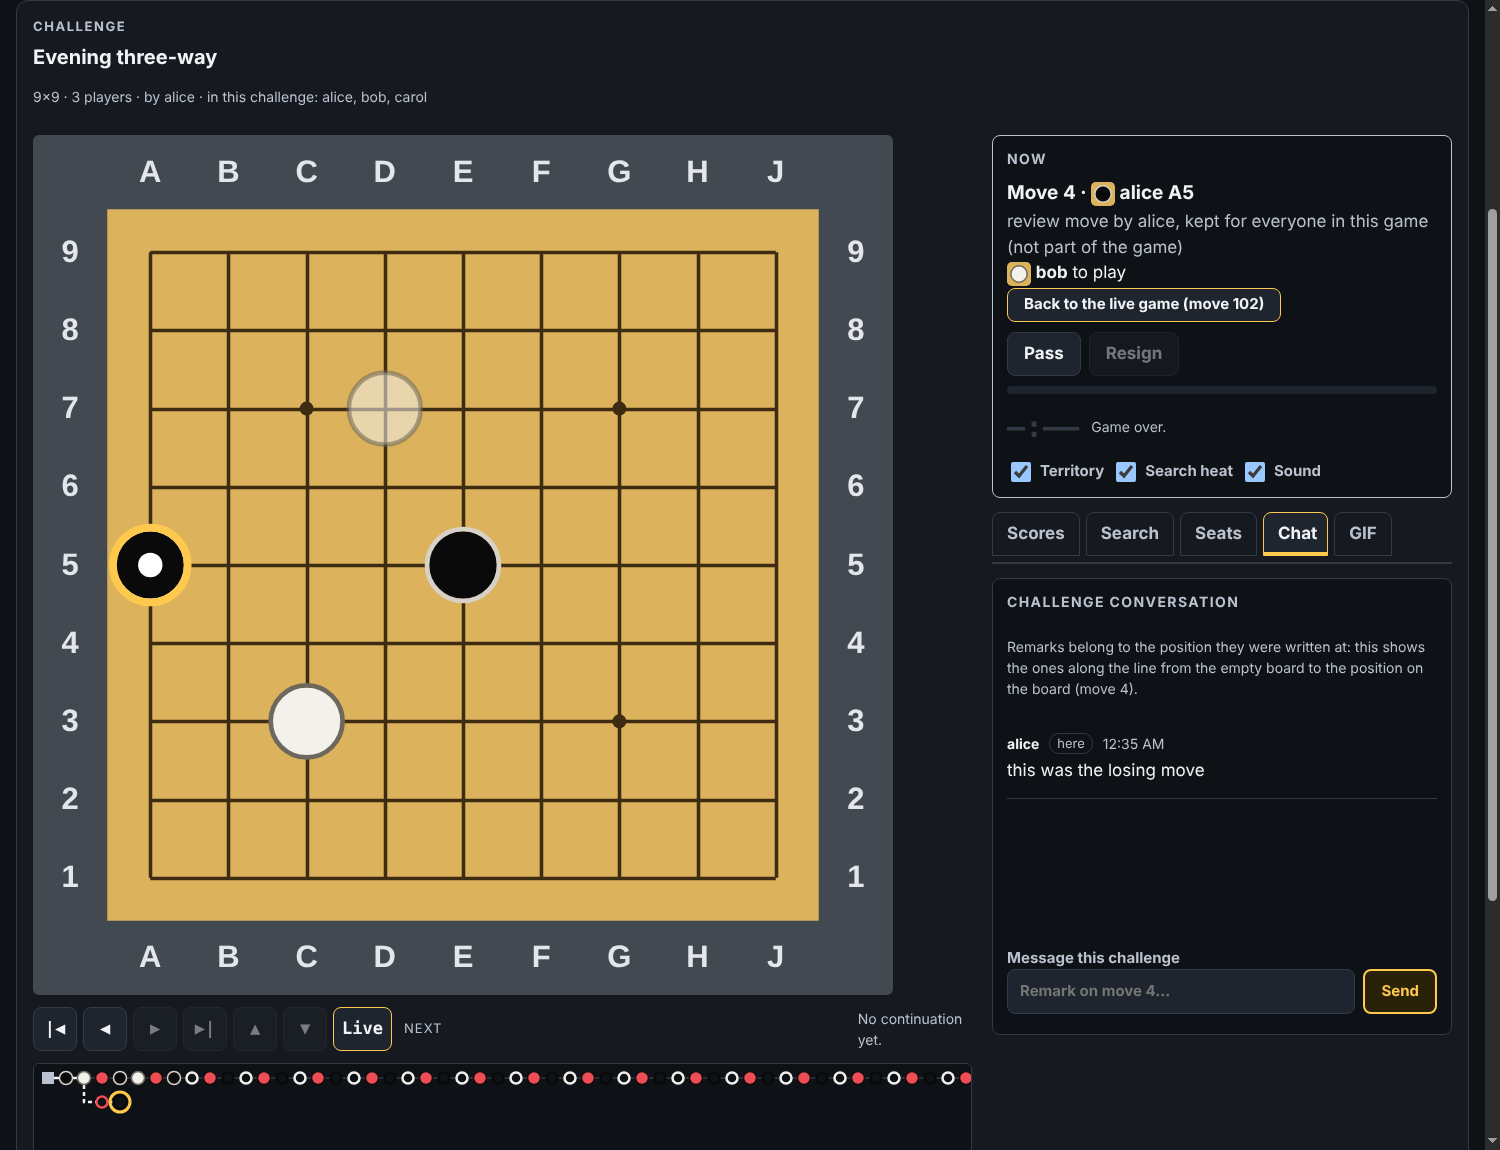
\includegraphics[width=\textwidth]{assets/tour/08a-review-chat.png}
\caption{Reviewing together, seen by alice. Steps: alice: Home, then → twice; alice: P, then C; alice: write a remark in Chat.}
\end{figure}
\clearpage

\section{Rooms and games as tabs}
Every room alice has open is a tab along the top, with + Rooms for finding and creating rooms; inside a room, the Lobby (its conversation and challenge list) comes first and every open game has its own tab. Tabs stay alive in the background: a game keeps its variations and analysis, and a tab shows a badge when a move or a merge waits for her or messages arrive. Responses only ever land in the tab that asked for them.

\begin{figure}[ht]
\centering
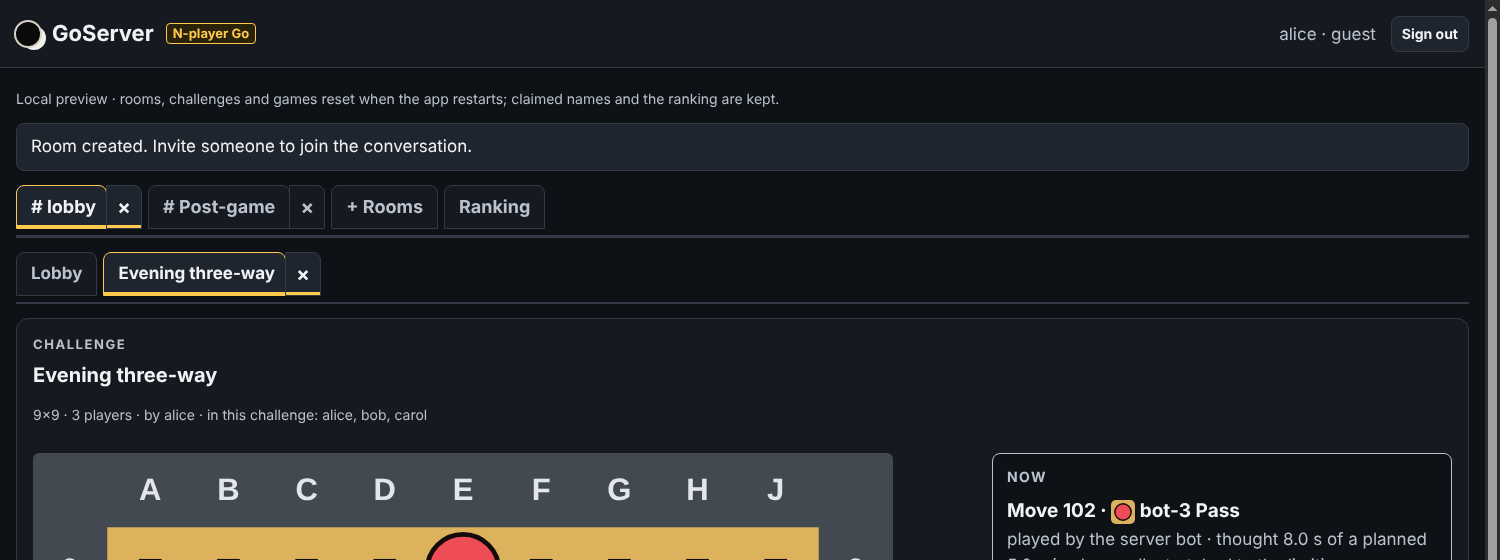
\includegraphics[width=\textwidth]{assets/tour/09-tabs.png}
\caption{Rooms and games as tabs, seen by alice. Steps: alice: + Rooms, create Post-game; alice: back to the lobby room tab.}
\end{figure}
\clearpage
